\section{Programme}
\subsection{Sidoc}
\subsubsection{Beschreibung}
Das Sidoc unterstützt Sie bei der Erstellung und Realisierung eines Sicherheitskonzeptes nach den Vorgaben des IT-Grundschutzes. Hierzu gehört die Bestimmung des Schutzbedarfs von IT-Anwendungen und IT-Systemen, die Erfassung und Darstellung des IST-Zustandes hinsichtlich der getroffenen Sicherheitsmaßnahmen, die Planung und Realisierung der SOLL-Zustandes sowie die SOLL-IST-Kontrolle bei der Realisierung. Darüber hinaus bietet das Sidoc eine integrierte Risikoanalyse für den über den IT-Grundschutz hinausgehenden Schutzbedarf.
Eine Kostenplanung und eine Revisionsverwaltung ergänzen das Sidoc zu einem vollwertigen Werkzeug für den IT-Sicherheitsbeauftragten und den IT-Sicherheitsberater.\cite{sidocDoku}
\\
Das Programm \textit{Sidoc} von \textit{2NET Carsten Lang} ist in einer kostenlosen Testversion unter \url{http://www.sidoc.info/} zu beziehen, welche den vollen Funktionsumfang bietet, jedoch ohne die Möglichkeit zu speichern.
\\
Die GUI von Sidoc ist mit seiner klassischen Baumstruktur stark an das Erscheinungsbild des BSI-GS-Tools angelehnt, zu sehen in einem Screenshot vom Programm in Abbildung ~\ref{sidocProgrammScreenshot}. In der Baumstruktur auf der linken Seite werden, wie im BSI-GS-Tool, die einzelnen zu modellierenden Bestandteile erschaffen und bei Bedarf verknüpft, auch mit entsprechenden Hovereffekten, wenn die Aktion nicht zulässig ist.
Komponenten, bei denen ein Schutzbedarf eingestellt werden kann, werden mit kleinen Schlüsselsymbolen gekennzeichnet. Unter $\rightarrow$IT-Ressourcen $\rightarrow$ Görlitz $\rightarrow$ G2 $\rightarrow$ R203 $\rightarrow$ WLAN sieht man auch, dass die drei gelben Schlüssel, welche hohen Schutzbedarf signalisieren, nach oben vererbt werden, wenn man einer unteren Komponente einen erhöhten Schutzbedarf zuweist. Dies kann auch nach einer Warnmeldung ignoriert werden.
Neben den Hardware Komponenten im unteren teil des Baumes gibt es im oberen Teil auch Personen(-gruppen), schützenswerte Informationen und Organisationseinheiten.
Auf der rechten Seite des Screenshots ist die Übersicht der durchzuführenden Maßnahmen. Der Übersicht ist zu entnehmen, welche Maßnahmen bereits durchgeführt wurden, noch durchzuführen sind und auch welche evtl. nicht durchführbar sind. ebenso ist zu sehen, welchen Einträgen des entsprechend verknüpften Kataloges die Maßnahme entstammt. Die angezeigten Maßnahmen beziehen sich auf das eben in der Baumstruktur selektierte Element, z.B. alle Maßnahmen, die ein Mitarbeiter zu bearbeiten hat, den man eben selektiert hat.
Neben einer Liste der durchzuführenden Maßnahmen kann man über die oberen Reiter auch andere Ansichten wählen, etwas die Kosten für Maßnahmen.
Zusätzlich zu diesen Listendarstellungen können manche Menüpunkte auch in grafischen Übersichten dargestellt werden, z.B. Prozesse oder IT-Ressourcen.
Alle möglichen Darstellungen oder auch Teile davon können in verschiedenen Formaten Exportiert werden.
\\
\begin{figure}
\label{sidocProgrammScreenshot}
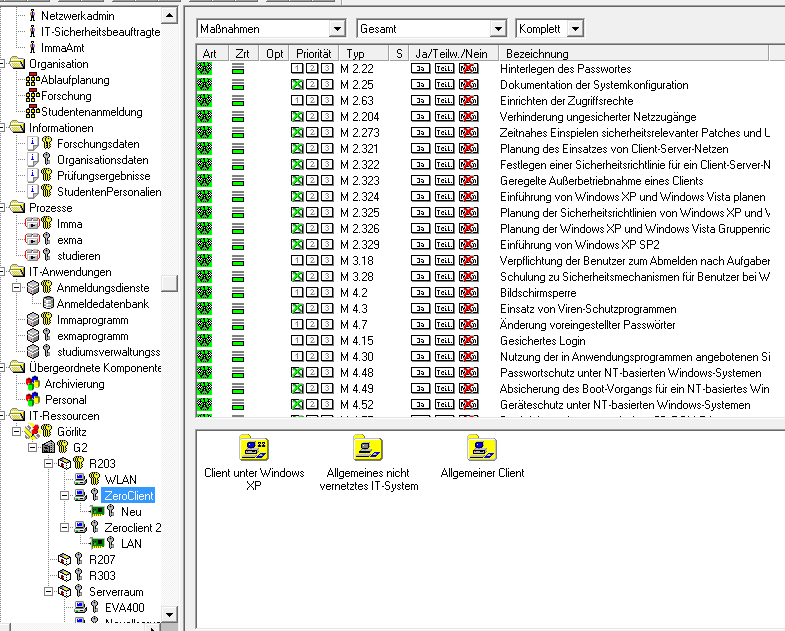
\includegraphics[scale=0.8]{images/sidocProgrammScreenshot.png} 
\caption{Screenshot von Sidoc mit teilen des Bsp. der HS}
\end{figure}
\\
\subsubsection{Bewertung}
\begin{itemize}
\item \textbf{Wizard:} Keine Wizards vorhanden
\item \textbf{Infrastrukturdarstellung:} Darstellung als Baumstruktur, ähnlich dem GS-Tool, jedoch mit anderen Bezeichnungen
\item \textbf{Netzpläne:} Sind in dem Programm enthalten, aber etwas schwer bedienbar.
\item \textbf{Prozessflüsse:} Sind vorhanden und übersichtlich, grafisch nicht sehr ansprechend aber Flüsse per Drag and Drop leicht zu bearbeiten. Leider sind keine mehrfachen Folgeprozesse möglich.
\item \textbf{Schnelles Einpflegen von Änderungen: } Änderungen können relativ schnell über die Arbeitsfläche eingebracht werden, auch wenn manche Optionen mehrfach in Reitern verschachtelt sind.
\item \textbf{Doppelseitige Verlinkungen:} In vollem Maß enthalten, teilweise auch optional, meistens per Drag and Drop zu bearbeiten.
\item \textbf{Vererbung:} Objekte erben den höchsten Schutzbedarf von mit ihnen verbundenen Objekten, werden davon abweichende Einstellungen vorgenommen, erscheint eine Warnung, aber man kann die Vererbung auch gezielt ignorieren.
\item \textbf{Gruppierungen:} Gruppierungen sind nicht vorgesehen.
\item \textbf{Aktuelle BSI-Standards:} Verschiedene Kataloge können importiert werden, wodurch sich u.A. die verfügbaren Bausteine ändern. Zu beachten ist jedoch der Punkt $\rightarrow$\textit{Pflege/Weiterentwicklung} weiter unten.
\item \textbf{Erweiterbarkeit der Klassifizierungen:} Schutzbedarfsstufen können angepasst werden und an manchen Stellen individuelle Klassen nach gewissen Vorgaben erstellt werden. Das ist jedoch limitiert durch die Grundbausteine und nicht für aalle Komponenten möglich. Im Tutorial wird die Möglichkeit zur Erstellung komplett unabhängiger neuer Bausteine beschrieben, konnte jedoch im Programm nicht nachvollzogen werden.
\item \textbf{Individuelle Beschreibungen:} Elemente können überall und nach belieben beschrieben werden.
\item \textbf{Sicherheitsverstöße markieren:} Entsprechend der gewählten Kataloge und der Art vorhandenen/genutzten Komponenten, werden alle relevanten Maßnahmen aufgelistet und entsprechend ihrer Sicherheit markiert und müssen bewusst als abgearbeitet markiert werden.
\item \textbf{Export von Berichten:} Große Anzahl von Exportmöglichkeiten. u.A. Risikobewertungen, Risikomatrizen, grafische Übersichten, etc.
\item \textbf{Bewertung des Sicherheitsstatus:} siehe $\rightarrow$\textit{Export von Berichten} und $\rightarrow$\textit{Sicherheitsverstöße markieren} weiter oben.
\item \textbf{GS-Tool import:} nein
\item \textbf{Sicherheit des Tools:} Benutzersteuerung, keine angaben zu Verschlüsselung o.Ä.
\item \textbf{Risikobewertung:} siehe $\rightarrow$\textit{Bewertung des Sicherheitsstatus}
\item \textbf{Verteiltes Arbeiten:} automatisches Speichern auf Server einstellbar in den Optionen.
\item \textbf{Rechtevergabe:} Rechtevergabe enthalten. Verschiedene Zugriffsstufen enthalten.
\item \textbf{Kosten:} Keine Angaben zu Lizenzkosten, da kein Kontakt erwidert wurde. Kostenlose Testversion mit vollem Funktionsumfang, jedoch ohne Speichermöglichkeit frei verfügbar.
\item \textbf{Zertifizierung:} Exporte von Berichten, die zur Zertifizierung notwendig sind, können erstellt werden.
\item \textbf{Support:} Keine Rückmeldung, weder Telefonisch noch per eMail oder Kontaktformular der Website.
\item \textbf{Dokumentation:} Nützliche Grundlagendokumentation, keine weiterführenden Tutorials.
\item \textbf{Marktpräsenz:} keine Angaben
\item \textbf{Nutzerkreis/Zielgruppe:} Keine spezielle Zielgruppe, stark orientiert am BSI-GS-Tool. durch individuelle Kataloge und Beschreibungen aber prinzipiell an verschiedene Bereiche anpassbar.
\item \textbf{Pflege/Weiterentwicklung:} Es ist anzunehmen, dass es nicht mehr weiterentwickelt bzw. gepflegt wird, da die Internetseite wiederholt nicht erreichbar war. (letzter Stand 01.02.2015: \url{http://www.sidoc.info/} nicht erreichbar)

\end{itemize}




\begin{table}[!htb]
%\centering
\begin{tabular}{|p{0.5\textwidth}|p{0.5\textwidth}|}
\hline 
Kriterium & Bewertung\\ 
\hline 
\textbf{GUI}& \\
\hline
Wizard & 0\\
\hline 
Infrastrukturdarstellung & 8 \\
\hline 
Netzpläne & 5 \\
\hline 
Prozessflüsse & 9 \\
\hline 
Schnelles Einpflegen von Änderungen & 9 \\
\hline
\textbf{Objektrelationen} & \\
\hline 
Doppelseitige Verlinkungen & 10 \\
\hline 
Vererbung & 10 \\
\hline 
Gruppierungen & 0 \\
\hline 
\textbf{Funktionalität} &\\
\hline 
Aktuelle BSI-Standards & 8 \\
\hline  
Erweiterbarkeit der Klassifizierungen & 4 \\
\hline 
Individuelle Beschreibungen & 10 \\
\hline 
Sicherheitsverstöße markieren & 10 \\
\hline
Bewertung des Sicherheitsstatus & 9 \\
\hline
Export von Berichten & 8 \\
\hline
BSI-Toolimport & 0 \\
\hline
Sicherheit des Tools an sich & 2 \\
\hline
Risikobewertung & 5 \\
\hline
\textbf{System}&  \\
\hline
Verteiltes Arbeiten & 2 \\
\hline
Rechtevergabe & 10 \\
\hline
Kosten & 0 \\
\hline
Support & 0 \\
\hline
Zertifizierung & 10 \\
\hline
Dokumentation & 4 \\
\hline
Marktpräsenz & 0 \\
\hline
Spezielle Zielgruppe & 0 \\
\hline
Pflege/Weiterentwicklung & 0 \\
\hline
\multicolumn{2}{c}{}\\
\hline
\textbf{Gesamt} & \\
\hline
Hochschuleinsatz & 52\%\\
\hline
Lehre & 55\%\\
\hline
\end{tabular} 
\caption{Bewertung: Sidoc}
\label{tab:BewertungSidoc}
\end{table}
\subsubsection{Auswertung}
Auf den ersten Blick ist \textit{Sidoc} ein passender Ersatz für das BSI-GS-Tool, da es einen ähnlichen Funktionsumfang und Arbeitsoberfläche bietet. Es ist durchweg übersichtlich gestaltet, bietet viele Einstellungsmöglichkeiten und lässt zu jeder Zeit Beschreibungen zu. Ebenso überzeugt die Integration der Vererbung. Die Darstellung der nötigen Maßnahmen ist sehr übersichtlich, gut filterbar und leicht Personen zuzuordnen.\\
Das größte und schwerwiegendste Problem ist, dass das Programm anscheinend nicht mehr gepflegt wird und somit für einen produktiven Einsatz an der Hochschule nicht in Frage kommt. Da die Testversion aber frei nutzbar ist, kann über eine Verwendung in der Lehre durchaus nachgedacht werden, da es zumindest das grundlegende Arbeiten mit einem GS-Tool gut wiedergibt und sehr übersichtlich und ohne große Einarbeitung genutzt werden kann.